%!TEX spellcheck = es_ES
\documentclass[12pt,a4paper,addpoints,answers]{exam}
%\documentclass[12pt,a4paper,addpoints]{exam}
\usepackage[utf8]{inputenc}
\usepackage[spanish]{babel}
\usepackage{adjustbox}
\usepackage{multirow}
\usepackage{graphicx}
\usepackage{tikz}
\usepackage{amsmath}
\usepackage{setspace}
\usepackage{afterpage}
\usepackage{ulem}
\usepackage{minted}
\usemintedstyle{pastie}

% Entidad-relación con TIKZ
\usetikzlibrary{er,shapes,positioning,calc}
\newcommand{\key}[1]{\underline{#1}}

\tikzset{weak entity/.style={entity ,double  distance =2pt}}
\tikzset{weak relationship/.style={relationship, double distance =2pt}}
\tikzset{
    -|/.style={to path={-| (\tikztotarget)}},
    |-/.style={to path={|- (\tikztotarget)}},
}

% Términos en castellano
\pointpoints{Punto}{Puntos}
\bonuspointpoints{Punto extra}{Puntos extra}
\renewcommand{\solutiontitle}{\noindent\textbf{Solución propuesta:}\enspace\\}
\chqword{Pregunta}
\chpgword{Página}
\chpword{Punto}
\chbpword{Punto extra}
\chsword{Obtenidos}
\chtword{Totales}
\hpword{Puntos:}
\hsword{Nota:}
\hqword{Ejercicio:}
\htword{Total:}

\pagestyle{headandfoot}
\firstpageheadrule
\runningheadrule
\firstpageheader{Bases de Datos I}{}{Segundo parcial\\Curso 2021/2022}
\runningheader{Bases de Datos I}{}{Segundo parcial\\Curso 2021/2022}
\firstpagefooter{}{}{\thepage\,/\,\numpages}
\runningfooter{}{}{\thepage\,/\,\numpages}

\begin{document}
\begin{center}
{\Huge Bases de Datos I -- Segundo parcial}\\
\vspace{2em}
{\Large SQL, normalización, acceso programático y seguridad}\\
\vspace{1em}
8 de junio de 2022
\end{center}

\begin{center}\textbf{Normativa de examen}\end{center}
\begin{itemize}
    \item No está permitido el uso de dispositivos móviles ni otros dispositivos electrónicos, así como libros ni apuntes.
    \item Durante el examen, los profesores podrán solicitar acreditar la identidad de los participantes en el mismo. Deberá tener en todo momento su Documento Nacional de Identidad y/o Carné de la UPM visible sobre la mesa.
    \item Deberá escribir su nombre y firma, \textbf{con bolígrafo}, en todas las hojas de las que consta el examen. El examen se resolverá \textbf{obligatoriamente a bolígrafo}.
    \item No se permite abandonar el aula de examen durante los \textbf{primeros 15 minutos}. Transcurrido este tiempo, no se permitirá entrar al examen.
    \item Este examen consta de \numquestions\ ejercicios para un total de \numpoints\ puntos.
    \item El examen tiene una duración máxima de \textbf{1.5 horas}.
    \item Según recoge la guía de la asignatura, es necesario obtener un 40\% de la nota de cada bloque para aprobar la asignatura por evaluación continua.
\end{itemize}
%\newpage

\begin{questions}
  \titledquestion{SQL y normalización}
  \label{question:sql}
  (\totalpoints\ puntos) \textbf{\large\thequestiontitle}
    
    Utilizando el siguiente modelo relacional resuelva las siguientes consultas usando \textbf{SQL}:
  
  \vspace{1em}
  \begin{center}
  \begin{adjustbox}{max height=0.3\textheight}
  \begin{tikzpicture}[relation/.style={rectangle split, rectangle split parts=#1, rectangle split part align=base, draw, anchor=center, align=center, text height=3mm, text centered}]\hspace*{-0.3cm}
  \node (alumnotitle) {\textbf{ALUMNO}};
  \node [relation=4, rectangle split horizontal, anchor=west, right=0.5cm of alumnotitle.east, anchor=west] (alumno)
    {\underline{Nmat}%
    \nodepart{two}   Nombre
    \nodepart{three} Apellidos
    \nodepart{four}  Correo};
  
  \node [anchor=north west,below=1.5cm of alumnotitle.west, anchor=north west] (asignaturatitle) {\textbf{ASIGNATURA}};
  \node [relation=4, rectangle split horizontal, anchor=west, right=0.5cm of asignaturatitle.east, anchor=west] (asignatura)
    {\underline{CodA}%
     \nodepart{two}   Nombre
     \nodepart{three} Créditos
     \nodepart{four}  Curso};

  \node [anchor=north west,below=1.5cm of asignaturatitle.west, anchor=north west] (cursatitle) {\textbf{CURSA}};
  \node [relation=5, rectangle split horizontal, anchor=west, right=0.5cm of cursatitle.east, anchor=west] (cursa)
    {\underline{CodA}%
     \nodepart{two}   \underline{Nmat}%
     \nodepart{three} \underline{CodG}%
     \nodepart{four}  \underline{Año}%
     \nodepart{five}  Nota};

  \node [anchor=north west,below=1.5cm of cursatitle.west, anchor=north west] (grupotitle) {\textbf{GRUPO}};
  \node [relation=4, rectangle split horizontal, anchor=west, right=0.5cm of grupotitle.east, anchor=west] (grupo)
    {\underline{CodG}%
     \nodepart{two}   Nombre
     \nodepart{three} Capacidad
     \nodepart{four}  Aula};

  \node [anchor=north west,below=1.5cm of grupotitle.west, anchor=north west] (impartetitle) {\textbf{IMPARTE}};
  \node [relation=4, rectangle split horizontal, anchor=west, right=0.5cm of impartetitle.east, anchor=west] (imparte)
    {\underline{CodP}%
     \nodepart{two}   \underline{CodG}%
     \nodepart{three} \underline{CodA}%
     \nodepart{four}  \underline{Año}};

  \node [anchor=north west,below=1.5cm of impartetitle.west, anchor=north west] (profesortitle) {\textbf{PROFESOR}};
  \node [relation=4, rectangle split horizontal, anchor=west, right=0.5cm of profesortitle.east, anchor=west] (profesor)
    {\underline{CodP}%
     \nodepart{two}   Nombre
     \nodepart{three} Apellidos
     \nodepart{four}  Despacho};

  % CLAVES FORANEAS
  \draw[-latex] (cursa.one north) -- ++(0,0.75) -| ($(asignatura.one south) + (-0.5,0)$);
  \draw[-latex] (cursa.two north) -- ++(0,0.30) -| ($(asignatura.four north) + (1,0.3)$) -| (alumno.one south);
  \draw[-latex] (cursa.three south) -- ++(0,-0.50) -| (grupo.one north);
  \draw[-latex] (imparte.one south) -- ++(0,-0.50) -| (profesor.one north);
  \draw[-latex] (imparte.two north) -- ++(0,0.50) -| (grupo.one south);
  \draw[-latex] (imparte.three north) -- ++(0,0.5) -| ($(asignatura.four south) + (0,-0.4)$) -| (asignatura.one south);
  \end{tikzpicture}
  \end{adjustbox}
  \end{center}
  
  \begin{parts}

  \part[1] Obtener el número de matrícula, nombre y apellidos del alumno o alumnos que han obtenido la mejor nota en cualquier asignatura que haya sido impartida por un profesor del despacho 1230.
  
  \begin{solutionorbox}
    \begin{minted}{sql}
SELECT a.Nmat, a.Nombre, a.Apellidos
FROM ALUMNO a INNER JOIN CURSA c ON a.Nmat = c.Nmat
    INNER JOIN GRUPO g ON c.CodG = g.CodG
    INNER JOIN IMPARTE i ON g.CodG = i.CodG
    INNER JOIN PROFESOR p ON i.CodP = p.CodP
WHERE p.Despacho = 1230 AND c.Nota >= ALL (
    SELECT c.Nota
    FROM CURSA INNER JOIN GRUPO g ON c.CodG = g.CodG
        INNER JOIN IMPARTE i ON g.CodG = i.CodG
        INNER JOIN PROFESOR p ON i.CodP = p.CodP
    WHERE p.Despacho = 1230
)
    \end{minted}
  \end{solutionorbox}
  
  \part[1] Obtener el código de profesor, nombre, apellidos y número total de alumnos a los que da clase cada uno de los profesores de la base de datos.
  
  \begin{solutionorbox}
    \begin{minted}{sql}
SELECT p.CodP, p.Nombre, p.Apellidos, COUNT(c.Nmat)
FROM PROFESOR p INNER JOIN IMPARTE i ON p.CodP = i.CodP
    INNER JOIN GRUPO g ON i.CodG = g.CodG
    INNER JOIN CURSA c ON g.CodG = c.CodG
GROUP BY p.CodP, p.Nombre, p.Apellidos
    \end{minted}
  \end{solutionorbox}
  
  \part[1] Diseñar una función que reciba el número de matricula de un alumno como parámetro y devuelva la nota media obtenida en todas las asignaturas que ha cursado.
  
  \begin{solutionorbox}
    \begin{minted}{sql}
DELIMITER //
CREATE FUNCTION f1 (num_mat VARCHAR(20))
RETURNS DECIMAL DETERMINISTIC
BEGIN
    DECLARE media DECIMAL;
    SELECT AVG(CURSA.Nota) INTO media
    FROM CURSA
    WHERE CURSA.Nmat = num_mat;
    
    RETURN(media);
END//
DELIMITER;
    \end{minted}
  \end{solutionorbox}
  
  \part[1] Diseñar un trigger que impida, mostrando un error, el borrado de un alumno si ha cursado más de cinco asignaturas distintas.
  
  \begin{solutionorbox}
    \begin{minted}{sql}
DELIMITER//
CREATE TRIGGER t1 BEFORE DELETE ON ALUMNO
FOR EACH ROW
BEGIN
    DECLARE cuenta INTEGER;
    SELECT COUNT(DISTINCT CodA) INTO cuenta
    FROM CURSA
    WHERE Nmat = OLD.Nmat;
    
    IF cuenta > 5 THEN
        SIGNAL SQLSTATE '02000'
        SET MESSAGE_TEXT = 'Error: alumno con más de 5 asignaturas';
    END IF;
END//
DELIMITER;
    \end{minted}
  \end{solutionorbox}

  %\newpage
  \part[1] \textbf{Normalización}: 
  
  ¿En qué forma normal se encuentra el siguiente modelo relacional representado como un esquema de relación de la forma $R=\left < T, L\right >$, siendo $T$ el conjunto de atributos, $L$ el conjunto de dependencias funcionales, $P$ el conjunto de atributos principales y $Q$ el conjunto de atributos no principales? \textbf{Justifique su respuesta}.
  
  \begin{align*}
  T &= \left \{ \textrm{Nmat}, \textrm{CodA}, \textrm{NotaText}, \textrm{NotaNum} \right \}\\
  L &= \left \{ \textrm{Nmat}\ \textrm{CodA} \longrightarrow \textrm{NotaNum}, \textrm{NotaNum}\longrightarrow \textrm{NotaText}\right \}\\
  P &= \left \{ \textrm{Nmat}, \textrm{CodA} \right \}\\
  Q &= \left \{ \textrm{NotaText}, \textrm{NotaNum} \right \}\\
  clave &= \left ( \textrm{Nmat}, \textrm{CodA} \right )
  \end{align*}
  
  \begin{solutionorbox}
    \begin{itemize}
        \item Está en primera forma normal porque cada atributo tiene un solo valor en cada tupla.
        \item Está en segunda forma normal porque ningún atributo no principal depende de un subconjunto de alguna clave.
        \item No está en tercera forma normal porque el atributo no principal $\textrm{NotaText}$ depende transitivamente de la clave.
        \item No está en forma normal Boyce-Codd porque no está en tercera forma normal.
    \end{itemize}
  \end{solutionorbox}
  \end{parts}
  
  %\newpage
  \titledquestion{Acceso programático}
  \label{question:programatico}
  (\totalpoints\ puntos) \textbf{\large\thequestiontitle}
  
  Completa los huecos numerados del código para realizar lo que se pide en cada problema.

  \begin{parts}
  \part[1] Usando el conector nativo de MySQL para Python, ejecutar la consulta y sacar por pantalla cada uno de los registros resultantes:
  
  \begin{minted}{python}
    import datetime
    import mysql.connector
    
    cnx = mysql._____(user='scott', database='employees') # 1
    cursor = cnx._____ # 2
    
    query = ("SELECT first_name, last_name, hire_date FROM employees "
             "WHERE hire_date BETWEEN %s AND %s")
    
    hire_start = datetime.date(1999, 1, 1)
    hire_end = datetime.date(1999, 12, 31)
    
    cursor._____(_____) # 3 y 4
    
    for _____ in cursor: # 5
      print("{}, {} was hired on {:%d %b %Y}".format(
        last_name, first_name, hire_date))
    
    cursor.close()
    cnx.close()
  \end{minted}
  
  \begin{solutionorbox}
    \begin{minted}{python}
import datetime
import mysql.connector

cnx = mysql.connector.connect(user='scott', database='employees')
cursor = cnx.cursor()

query = ("SELECT first_name, last_name, hire_date FROM employees "
         "WHERE hire_date BETWEEN %s AND %s")

hire_start = datetime.date(1999, 1, 1)
hire_end = datetime.date(1999, 12, 31)

cursor.execute(query, (hire_start, hire_end))

for (first_name, last_name, hire_date) in cursor:
  print("{}, {} was hired on {:%d %b %Y}".format(
    last_name, first_name, hire_date))

cursor.close()
cnx.close()
    \end{minted}
  \end{solutionorbox}
  
  %\newpage
  \vspace{1em}
  \part[1] Completa los huecos del código para definir con SQLAlchemy ORM dos clases que se corresponden con las tablas del siguiente modelo:
  
  \begin{figure}[h]
      \centering
      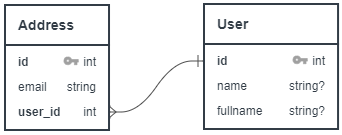
\includegraphics{erd.png}
  \end{figure}
  
  \begin{minted}{python}
class User(Base):
    __tablename__ = "user_account"
    id = Column(_____) # 1
    name = Column(String(30))
    fullname = Column(String)

class Address(Base):
    __tablename__ = "address"
    id = Column(_____) # 2
    email_address = Column(_____) # 3
    user_id = Column(_____) # 4
    user = relationship(_____) # 5
  \end{minted}
  
  \begin{solutionorbox}
    \begin{minted}{python}
class User(Base):
    __tablename__ = "user_account"
    id = Column(Integer, primary_key=True)
    name = Column(String(30))
    fullname = Column(String)

class Address(Base):
    __tablename__ = "address"
    id = Column(Integer, primary_key=True)
    email_address = Column(String, nullable=False)
    user_id = Column(Integer, ForeignKey("user_account.id"), nullable=False)
    user = relationship("User", back_populates="addresses")
    \end{minted}
  \end{solutionorbox}
  
  \vspace{1em}
  \part[\half] Explica brevemente cómo funciona el ORM de SQLAlchemy y qué ventajas aporta a los desarrolladores.
  
  \begin{solutionorbox}
    Un ORM realiza automáticamente un mapeado entre las filas de tablas en una base de datos y las instancias de distintas clases de Python. Permite a los desarrolladores abstraerse de la capa de persistencia de los datos de sus aplicaciones, puesto que las inserciones, actualizaciones, borrados y definición del esquema se realiza automáticamente por parte del ORM.
  \end{solutionorbox}
  
  \end{parts}
  
  \titledquestion{Seguridad}
  \label{question:seguridad}
  (\totalpoints\ puntos) \textbf{\large\thequestiontitle}
  
  Elige la respuesta correcta (opción única). Una respuesta incorrecta resta $\frac{1}{6}$ puntos.
  
  \begin{parts}
  
  \part[\half] MySQL utiliza la seguridad basada en \underline{\hspace{3cm}} para todas las conexiones, consultas y otras operaciones que los usuarios pueden intentar realizar:
  
  \begin{choices}
     \choice Esquemas de administrador
     \choice Algoritmos de encriptación
     \choice Preferencias de usuario
     \choice Listas de control de acceso
  \end{choices}
  
  \begin{solutionorbox}
    Listas de control de acceso
  \end{solutionorbox}
  
  \part[\half] Necesita hacer que su sistema MySQL sea seguro contra los atacantes. ¿Qué se supone que \textbf{no} debe hacer?:
  
  \begin{choices}
     \choice Ejecutar el servidor MySQL como un usuario normal.
     \choice Conceder el privilegio PROCESS o SUPER a otros usuarios.
     \choice Ejecutar el servidor MySQL como el usuario root de unix.
     \choice Usar el protocolo comprimido.
  \end{choices}
  
  \begin{solutionorbox}
    Ejecutar el servidor MySQL como el usuario root de unix.
  \end{solutionorbox}
  
  \part[\half] ¿A qué aspecto de la seguridad de MySQL corresponde la capacidad del servidor de almacenar los nombres de usuario y sus contraseñas encriptadas en una tabla?:
  
  \begin{oneparchoices}
     \choice Autenticación
     \choice Autorización
     \choice Encriptación
     \choice Auditoría y Firewall
  \end{oneparchoices}
  
  \begin{solutionorbox}
    Autenticación
  \end{solutionorbox}
  
  \part[\half] ¿Qué afirmación es falsa en relación a la encriptación de MySQL?:
  
  \begin{choices}
     \choice La comunicación entre cliente y servidor se encripta mediante certificados SSL/TLS.
     \choice La información contenida en las tablas se puede encriptar.
     \choice La comunicación cliente-servidor está encriptada por defecto, por lo que no se permite una conexión sin cifrar.
     \choice La encriptación cliente-servidor impide que un atacante pueda obtener los datos a traves de la red.
  \end{choices}
  
  \begin{solutionorbox}
    La comunicación cliente-servidor está encriptada por defecto, por lo que no se permite una conexión sin cifrar.
  \end{solutionorbox}
  
  \part[\half] ¿Cuál es el ataque más frecuente a una base de datos?:
  
  \begin{oneparchoices}
     \choice Fuerza bruta.
     \choice Inyección SQL.
     \choice Denegación de servicio.
     \choice Robo de credenciales.
  \end{oneparchoices}
  
  \begin{solutionorbox}
    Inyección SQL
  \end{solutionorbox}
  
  \end{parts}
\end{questions}
\end{document}